% !Mode:: "TeX:UTF-8"

\BiChapter{基于格的微基站部署的性能分析}{architecture and system model}

本章介绍基于格的微基站部署,
这也是网络部署的一种基本的方法。
该方法分为两个步骤,首先在服务区域~$\mathcal{D}$~中选定固定格点,
然后在选定的格点上部署微基站。
常见的基于格的微基站部署有环形部署和方格部署,
在进行分析之前,首先对网络中的关键性能指标进行描述,
然后分别对上述不同的基站部署的拓扑结构进行介绍和性能分析。

\BiSection{超密集组网通信的性能指标}{matrices}
本小节介绍衡量超密集组网的通信性能的主要指标,其中包括信干噪比、遍历容量、覆盖率和单位面积谱效率。

\BiSubsection{信干噪比}{SINR}

可靠性和有效性一直是评定通信性能的一个重要指标。其中有效性可以通过网络的信道容量进行衡量。而网络的信道容量是一个直接与信干噪比有关的量。
信干噪比的表达式如~(\ref{SINR})~所示:
\begin{equation}\label{SINR}
  \mathrm{SINR}=\frac{S}{I+N}
\end{equation}
其中~$S$~为通信链路中接收机的接收功率,~$I$~为其他的通信链路对该通信链路所造成的干扰。$\mathrm{SINR}$~表示该通信链路的信干燥比。

超密集组网区域用户与基站之间距离比较近,因此干扰占有几乎全部的比重,反之噪声的影响几乎可以忽略不计。也就是说,密集无线网络是一个干扰受限的信道。其信干比近似等于信干燥比。信干比的表达式如~(\ref{SIR})~:
\begin{equation}\label{SIR}
  \mathrm{SIR}=S/I
\end{equation}
其中~$\mathrm{SIR}$~表示该通信链路的信干比。
\BiSubsection{用户的遍历容量}{ASE}
给定一个用户的接收信干比,即可以求出一个用户的遍历容量,在平稳的瑞利信道下,用户的遍历容量如式~\ref{e_capacity_formular}~所示:
\begin{equation}\label{e_capacity_formular}
  C_{Rayleigh} = \int_{0}^{\infty} B \log_2(1+\mathrm{SINR}(h)) f(h) \mathrm{d} h
\end{equation}
其中~$C_{Rayleigh}$~为瑞利信道的遍历容量,~$f(h)$~为~$h$~的概率密度分布函数,$B$~为信道的带宽。信道的遍历容量表示一个用户在一段时间内,遍历所有可能性下的信道容量的统计平均值。
因为信道为瑞利信道,因此在固定位置上的用户,由于受到了信道系数的影响,其信干噪比在不同的时间点上也是不同的,又由于瑞利信道是平稳的信道,
因此可以采用遍历所有信道系数的可能性得到的统计均值代替时间上的遍历,用~$\mathrm{SINR}(h))$~表示。

遍历容量可以反应一个用户在一段时间内通信的有效性,是反应网络性能的重要指标。

\BiSubsection{区域覆盖率}{Coverage}
为保证用户的服务质量与速率要求,用户的接收信干比需要维持在一个固定的门限上,而到底有多少用户在该时刻上有很好的信干比,或者说在瞬时上能达到所要求的信干比的用户一共有多少呢?区域覆盖率是评定的有效的指标。
区域覆盖率的定义如~(\ref{pc})~所示:
\begin{equation}\label{pc}
  p_c(T) = \mathbb{P}[\mathrm{SINR}>T]
\end{equation}
其中~$T$~为给定的信干噪比的门限,~$\mathrm{SINR}$~为通信链路的信干噪比,$\mathbb{P}$~表示概率。根据定义,可对其物理意义做出以下的三种解释:

 (1)~服务用户的信干噪比为以上的概率。

 (2)~信干噪比为以上的用户占总用户的百分比。

 (3)~信干噪比为以上的区域占总区域的百分比。

覆盖率是评定无线网络性能的一个重要的概念,并且根据覆盖率,可以很容易的得到有能达到给定的速率要求在整个区域中的所有用户的占比。
同时该物理量也是单位区域上信干噪比的概率分布函数的补函数。
\BiSubsection{区域面积谱效率}{ASE}

香农定理给出了通信系统的理论容量上界\citeup{TheMathematicalTheoryOfCommunication},表达式如~(\ref{shannon})~所示:
\begin{equation}\label{shannon}
  C = B \log_2(1+\mathrm{SINR})
\end{equation}

式~(\ref{shannon})~中,~$C$~ 代表理论的容量的上界也即系统最大的传输速率, $B$ 代表信道的带宽, ~$\mathrm{SINR}$~ 代表接收端信号的信干噪比。
香农定理可以解释现代各种无线制式由于带宽不同,所支持的单载波最大吞吐量的不同。香农公式表达了在给定带宽下,噪声和干扰都服从高斯分布的情况下,系统所能达到的理论最大容量。

频谱效率的定义为单位带宽上所能承载的最大的吞吐量,如~(\ref{SE})~所示:
\begin{equation}\label{SE}
\eta_{SE}=C/B=\log_2(1+\mathrm{SINR})
\end{equation}
上式中~$C/B$~就是单位带宽的容量,单位为~$bps/\mathrm{Hz}$~体现信道链路的传输性能。式~(\ref{SE})~给出了理论上频谱效率的理论最大值。

在密集热点区域无线网络的场景中,单个链路的容量已经不再是衡量一个网络的好坏的唯一指标,在超密集热点区域无线网络的场景中,还要考虑在一段时间内,网络中服务的用户的和容量。
同时,考虑到不同区域上的频谱效率相差可能非常悬殊。因此在密集热点的网络环境下,频谱效率将不能够完全反映整个区域的无线网络的性能,
取而代之的是单位面积谱效率这一物理量,其定义为在单位面积上的频谱效率,表达式如~(\ref{ASE})~所示:
\begin{equation}\label{ASE}
  \eta_{ASE}=C/(B\cdot S) = \lambda\mathbb{E}[\log_2(1+\mathrm{SINR})]
\end{equation}
单位为~$bps/\mathrm{Hz}/\mathrm{m}^2$~。其中~$\lambda$~为服务区域内基站的密度。区域面积谱效率的物理意义为单位面积上所承载的平均的和容量。

\BiSection{环形的基站部署}{Defination of UDNs}

\BiSubsection{环形的基站部署的拓扑结构}{Defination of UDNs}
环形基站部署将基站部署在一个圆环上,其特别适合大型比赛场馆,大型演唱会等场景下的基站部署。
环形的基站部署方法的示意图如图~\ref{single_circle_bs_show}~所示,
在区域~$\mathcal{D}$~上,选定半径~$R$,在半径为~$R$~的圆上均匀的部署~$N$~个基站,
在图~\ref{single_circle_bs_show}~中,
$\mathcal{D}$~为一个~$100\mathrm{m}\times 100 \mathrm{m}$~的区域,
部署基站的半径大小~$R=30\mathrm{m}$,基站的个数~$N=12$~个。
\begin{figure}[htbp]
\centering
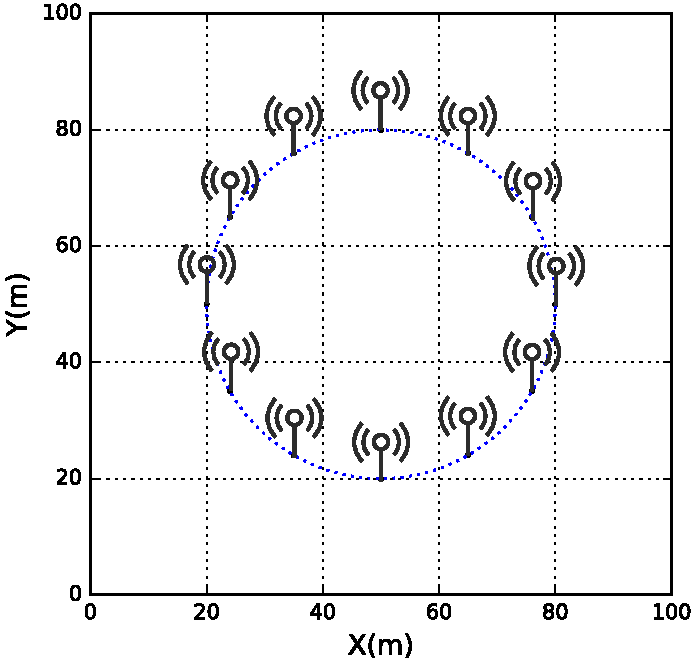
\includegraphics[width = 0.62\textwidth]{single_circle_bs_station.pdf}
\caption{环形基站部署的拓扑结构示意图}\vspace{-0.5em}
\label{single_circle_bs_show}
\end{figure}
若微基站同时同频的传送信息,
则由于在中心处的用户距所有基站的距离均比较近,
因此在未采用任何基站协作的前提下,若以就近原则选择服务的基站,
处在中心处的用户受到除服务基站以外的其他基站的干扰非常严重,
但由于处在距离环比较近的用户距离服务基站的距离较近,因此接收信号较强,
用户的接收信干噪比较好,处在圆环区域附近的用户的覆盖性能是较好的。
在环形基站的部署当中,基站的个数~$N$~和圆环的大小~$R$~以及服务区域的面积的大小均是
有关系的,由于网络模型复杂,不易对网络的各个性能求出闭合解,
但是可以用蒙特卡洛仿真的方法分析网络的性能,下面对在不同的参数条件下的基站环形部署的性能进行分析。

\BiSubsection{环形的基站部署的遍历容量}{Defination of UDNs}
对环形基站的遍历容量分布图进行蒙特卡洛仿真分析,
仿真的参数表如表~\ref{single_circle_sinr_sim_para}~所示,
\begin{table}[htbp]
\caption{遍历容量的热力分布图的仿真参数}
\label{single_circle_sinr_sim_para}
\vspace{0.5em}\centering\wuhao
\begin{tabular}{cccc}
\toprule[1.5pt]
参量 & & & 设置 \\
\midrule[0.5pt]
区域~$\mathcal{D}$~的大小  & & & ~$100\mathrm{m} \times 100 \mathrm{m}$~ \\
信道的类型 & & &  瑞利衰落信道\\
基站的个数~$N$~ & & &  12\\
圆环的半径~$R$~ & & &  ${30\mathrm{m}}$\\
信道衰落系数~$\alpha$~  & & & 2,~4\\
\bottomrule[1.5pt]
\end{tabular}
\end{table}
该仿真主要反应了瑞利信道下的区域内的各个位置的遍历容量的特性,
而遍历容量是一个与信干比相关的量,
因此仿真结果可以反应每个区域上的信干比的特性。
基站的个数、圆环的大小、区域的大小固定,通过遍历容量热力分布图可以得到信道衰落系数对网络的遍历容量的性能的影响,
采用蒙特卡洛仿真,得到的结果如图~\ref{single_circle_e_capacity_show}~所示,
\begin{figure}[htbp]
\centering
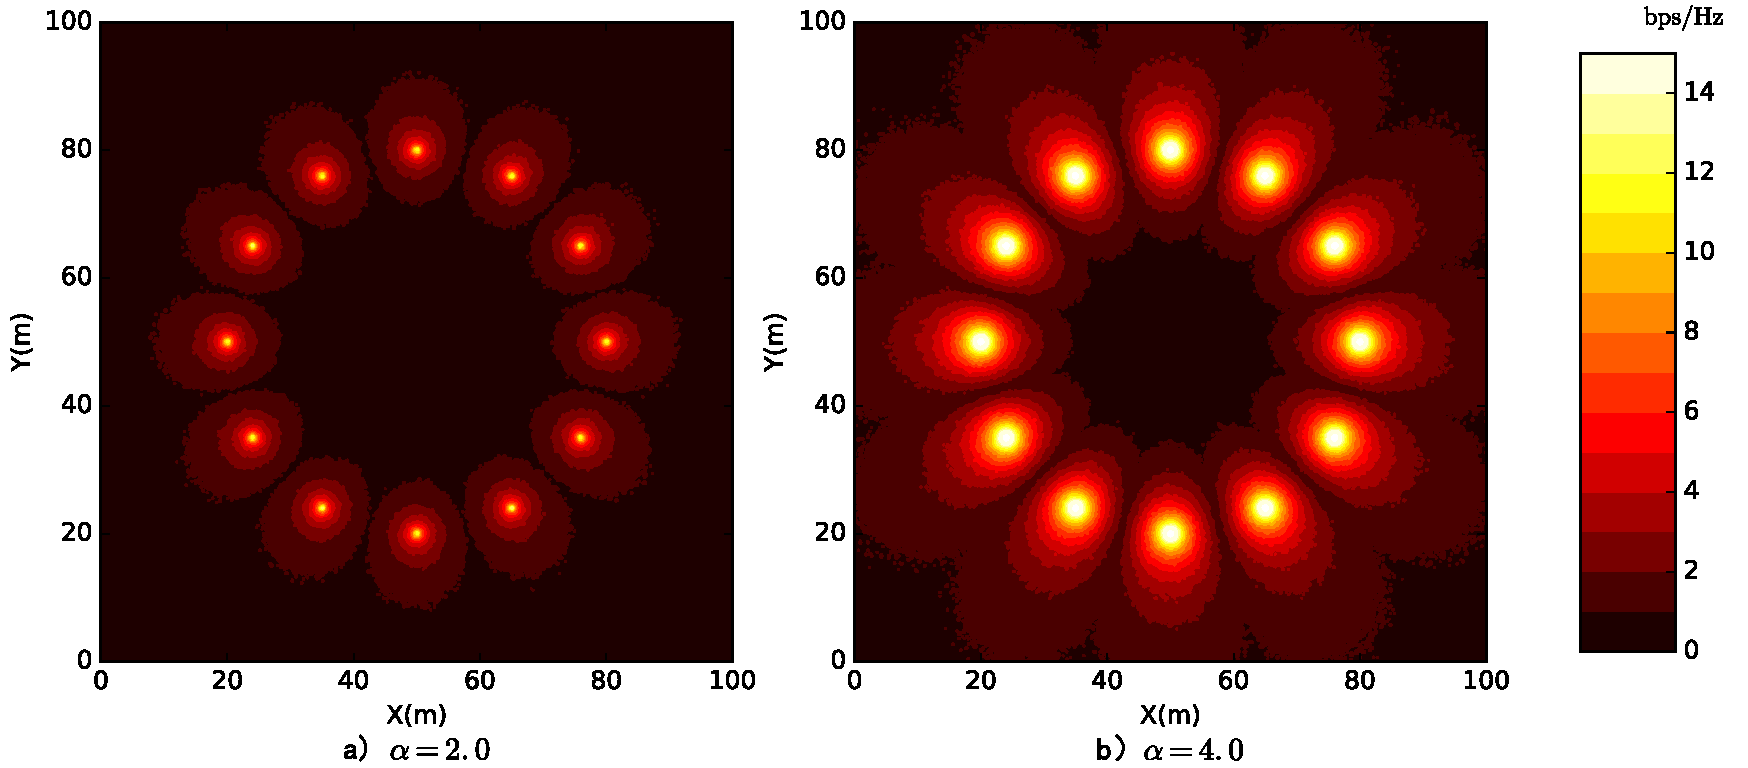
\includegraphics[width = 0.98\textwidth]{single_circle_e_capacity_show_30_12.pdf}
\caption{环形基站部署的遍历容量热力图:~(左)~$\alpha=2$~(右)~$\alpha=4$}\vspace{-0.5em}
\label{single_circle_e_capacity_show}
\end{figure}
可以看到距离服务基站较近的用户的遍历容量较好,
当~$\alpha=4$~时,距离微基站大概~$3\mathrm{m}$~以内的用户的遍历容量均大于~$10\mathrm{bps/Hz}$。
整个区域的热力分布图呈现辐射状,信道衰减系数大的辐射的更远,处在中心处的用户的性能很差,
遍历容量小于~$1\mathrm{bps/Hz}$。

\BiSubsection{环形的基站部署的覆盖率的性能分析}{Defination of UDNs}
我们在上一小节讨论了路径损耗因子对性能的影响,
接下来对网络的覆盖率性能采用蒙特卡洛仿真分析,对网络的覆盖率性能进行分析,
主要分析环形基站部署的两个重要指标,即圆环的半径~$R$和基站的个数~$N$对基站的覆盖率的影响。
同时,由于用户在区域内的分布不一定是均匀的,因此需要对不同用户的分布情况进行分析,
考虑用户的分布~$\Psi$~分别为随机分布和以微基站的位置坐标为均值的二维高斯分布的情况。
仿真的参数表如表~\ref{single_circle_pc_sim_para}~所示,
\begin{table}[htbp]
\caption{覆盖率的仿真参数}
\label{single_circle_pc_sim_para}
\vspace{0.5em}\centering\wuhao
\begin{tabular}{cccc}
\toprule[1.5pt]
参量 & & & 设置 \\
\midrule[0.5pt]
区域~$\mathcal{D}$~的大小  & & & ~$100\mathrm{m} \times 100 \mathrm{m}$ \\
信道的类型 & & &  瑞利衰落信道\\
基站的个数~$N$~ & & &  8, 16\\
圆环的半径~$R$~ & & &  ${30\mathrm{m}},{50\mathrm{m}}$\\
用户的分布~$\Psi$~ & & & 随机分布,二维高斯分布\\
二维高斯分布的标准差~$\sigma$~ & & & ${5\mathrm{m}}$\\
信道衰落系数~$\alpha$~  & & & 4\\
\bottomrule[1.5pt]
\end{tabular}
\end{table}
下面通过仿真的方法分析上述主要参数对覆盖率性能的影响。
将表中的半径参数~$R$~和基站个数参数~$N$~进行全组合,
得到~4~种情况,
覆盖率性能的曲线如图~\ref{pc_random_single_circle_r_n}~所示,
在用户分布为随机分布的情况下的覆盖率仿真曲线如图~\ref{pc_random_single_circle_r_n}~(a)所示,
\begin{figure}[htbp]
\centering
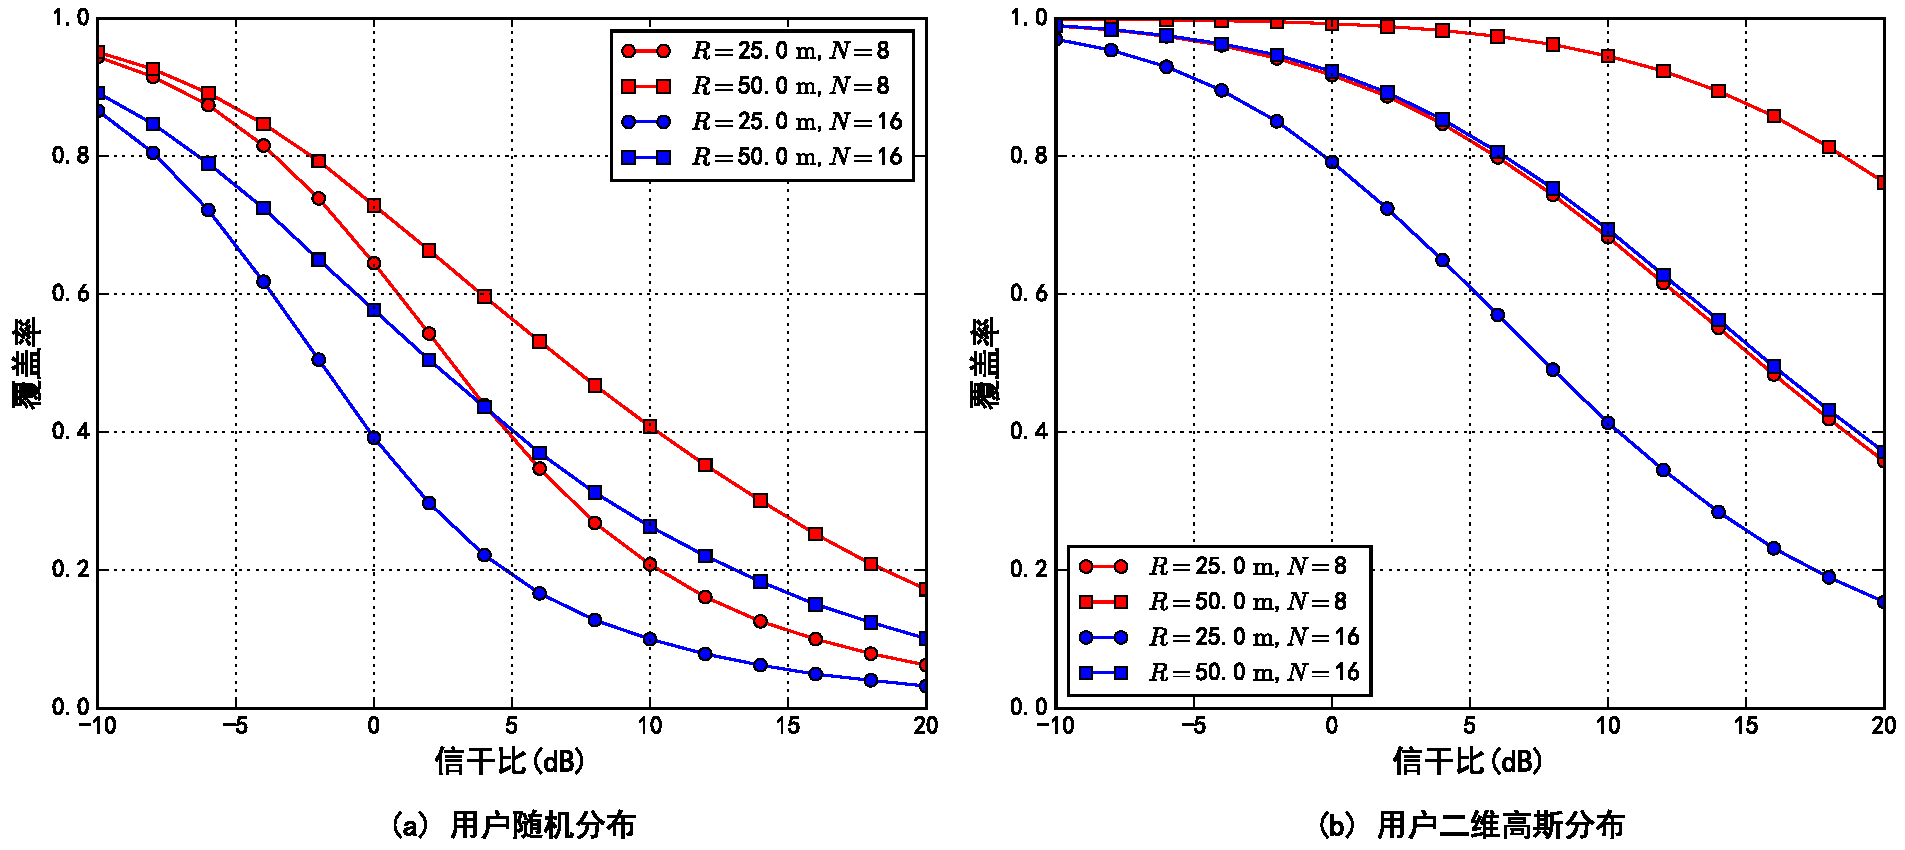
\includegraphics[width = 0.90\textwidth]{pc_random_single_circle_r_n.pdf}
\caption{环形基站部署的覆盖率性能曲线}\vspace{-0.5em}
\label{pc_random_single_circle_r_n}
\end{figure}
通过性能曲线可以看出,总体来讲,基站数目~$N$~越多,部署基站的半径~$R$~越小,则覆盖率的性能越差,
低信干比门限下,受半径~$R$~影响更强烈,
高信干比门限下,受基站数~$N$~影响更强烈。
在用户分布为以基站坐标为均值的混合二维高斯分布情况下的覆盖率仿真曲线,
如图~\ref{pc_random_single_circle_r_n}~(b)所示,
同样是基站数目~$N$~越多,部署基站的半径~$R$~越小,则覆盖率的性能越差,
但用户为混合二维高斯分布情况下基站数~$N$~和半径~$R$~对网络覆盖率性能的影响大致上相同,
$N=8,R=25\mathrm{m}$~时的情况和$N=16,R=50\mathrm{m}$~时,网络的覆盖率性能大体上是相同的。
也可以看到此时网络的覆盖率性能和用户分布随机的情况相比有了明显的好转,
当~$N=8,R=50\mathrm{m}$~时,网络在$5\mathrm{dB}$的覆盖率甚至接近1。

图~\ref{pc_random_single_circle_r_n}~给出了特定的~$N$~和~$R$~的情况下的覆盖率与信干比的关系曲线,
从曲线中,我们可以看出当~$N=8, ~12$~和~$R=25.0,~50.0\mathrm{m}$~下,网络的覆盖率的具体情况,
但曲线并不能反应覆盖率随~$N$~和~$R$~的变化的关系,
为了得到覆盖率与~$N$~和~$R$~的关系,
选定信干比的典型值~$0\mathrm{dB}$,$3\mathrm{dB}$,$5\mathrm{dB}$时,
可以得到覆盖率与~$R$~和~$N$~的关系的曲面图,
仿真的参数表如表~\ref{pc_random_single_circle_r_n_table}~所示,
\begin{table}[htbp]
\caption{覆盖率与~$R$~和~$N$~的关系的仿真参数}
\label{pc_random_single_circle_r_n_table}
\vspace{0.5em}\centering\wuhao
\begin{tabular}{cccc}
\toprule[1.5pt]
参量 & & & 设置 \\
\midrule[0.5pt]
区域~$\mathcal{D}$~的大小  & & & ~$100\mathrm{m} \times 100 \mathrm{m}$ \\
信道的类型 & & &  瑞利衰落信道\\
基站的个数~$N$~ & & &  $2\sim20$\\
圆环的半径~$R$~ & & &  $1.0\sim 50\mathrm{m}$\\
信干比门限~$\delta$~  & & & ~$0\mathrm{dB}$,$3\mathrm{dB}$,$5\mathrm{dB}$\\
用户的分布~$\Psi$~ & & & 随机分布,二维高斯分布\\
二维高斯分布的标准差~$\sigma$~ & & & ${5\mathrm{m}}$\\
信道衰落系数~$\alpha$~  & & & 4.0\\
\bottomrule[1.5pt]
\end{tabular}
\end{table}
仿真得到的曲面图如图~\ref{pc_random_single_circle_r_n_face}~所示,
可以看到当用户的分布为随机分布的情况下,覆盖率随着基站数的变化大体上是逐渐降低的,
与之前讨论得到的结果是一致的,但随着半径的变化不再是单调的,说明覆盖率的性能随着部署半径的增大先增大后减小,
最优的部署半径的值大概为~$R = 40~\mathrm{m}$~左右。
当用户的分布服从混合二维高斯分布的情况下,覆盖率随着基站数目~$N$~越多,部署基站的半径~$R$~越小,则覆盖率的性能越差,
且二者的对覆盖率的影响程度基本相同,与之前分析的结果是一致的。
在实际的部署中,可以根据覆盖率的需求合理的设定信干比门限,在设定了信干比门限的情况下,
通过图~\ref{pc_random_single_circle_r_n_face}~即可得到环形基站部署方法下使覆盖率性能达到最优的基站数~$N$~
和部署半径~$R$。
\begin{figure}[htbp]
\centering
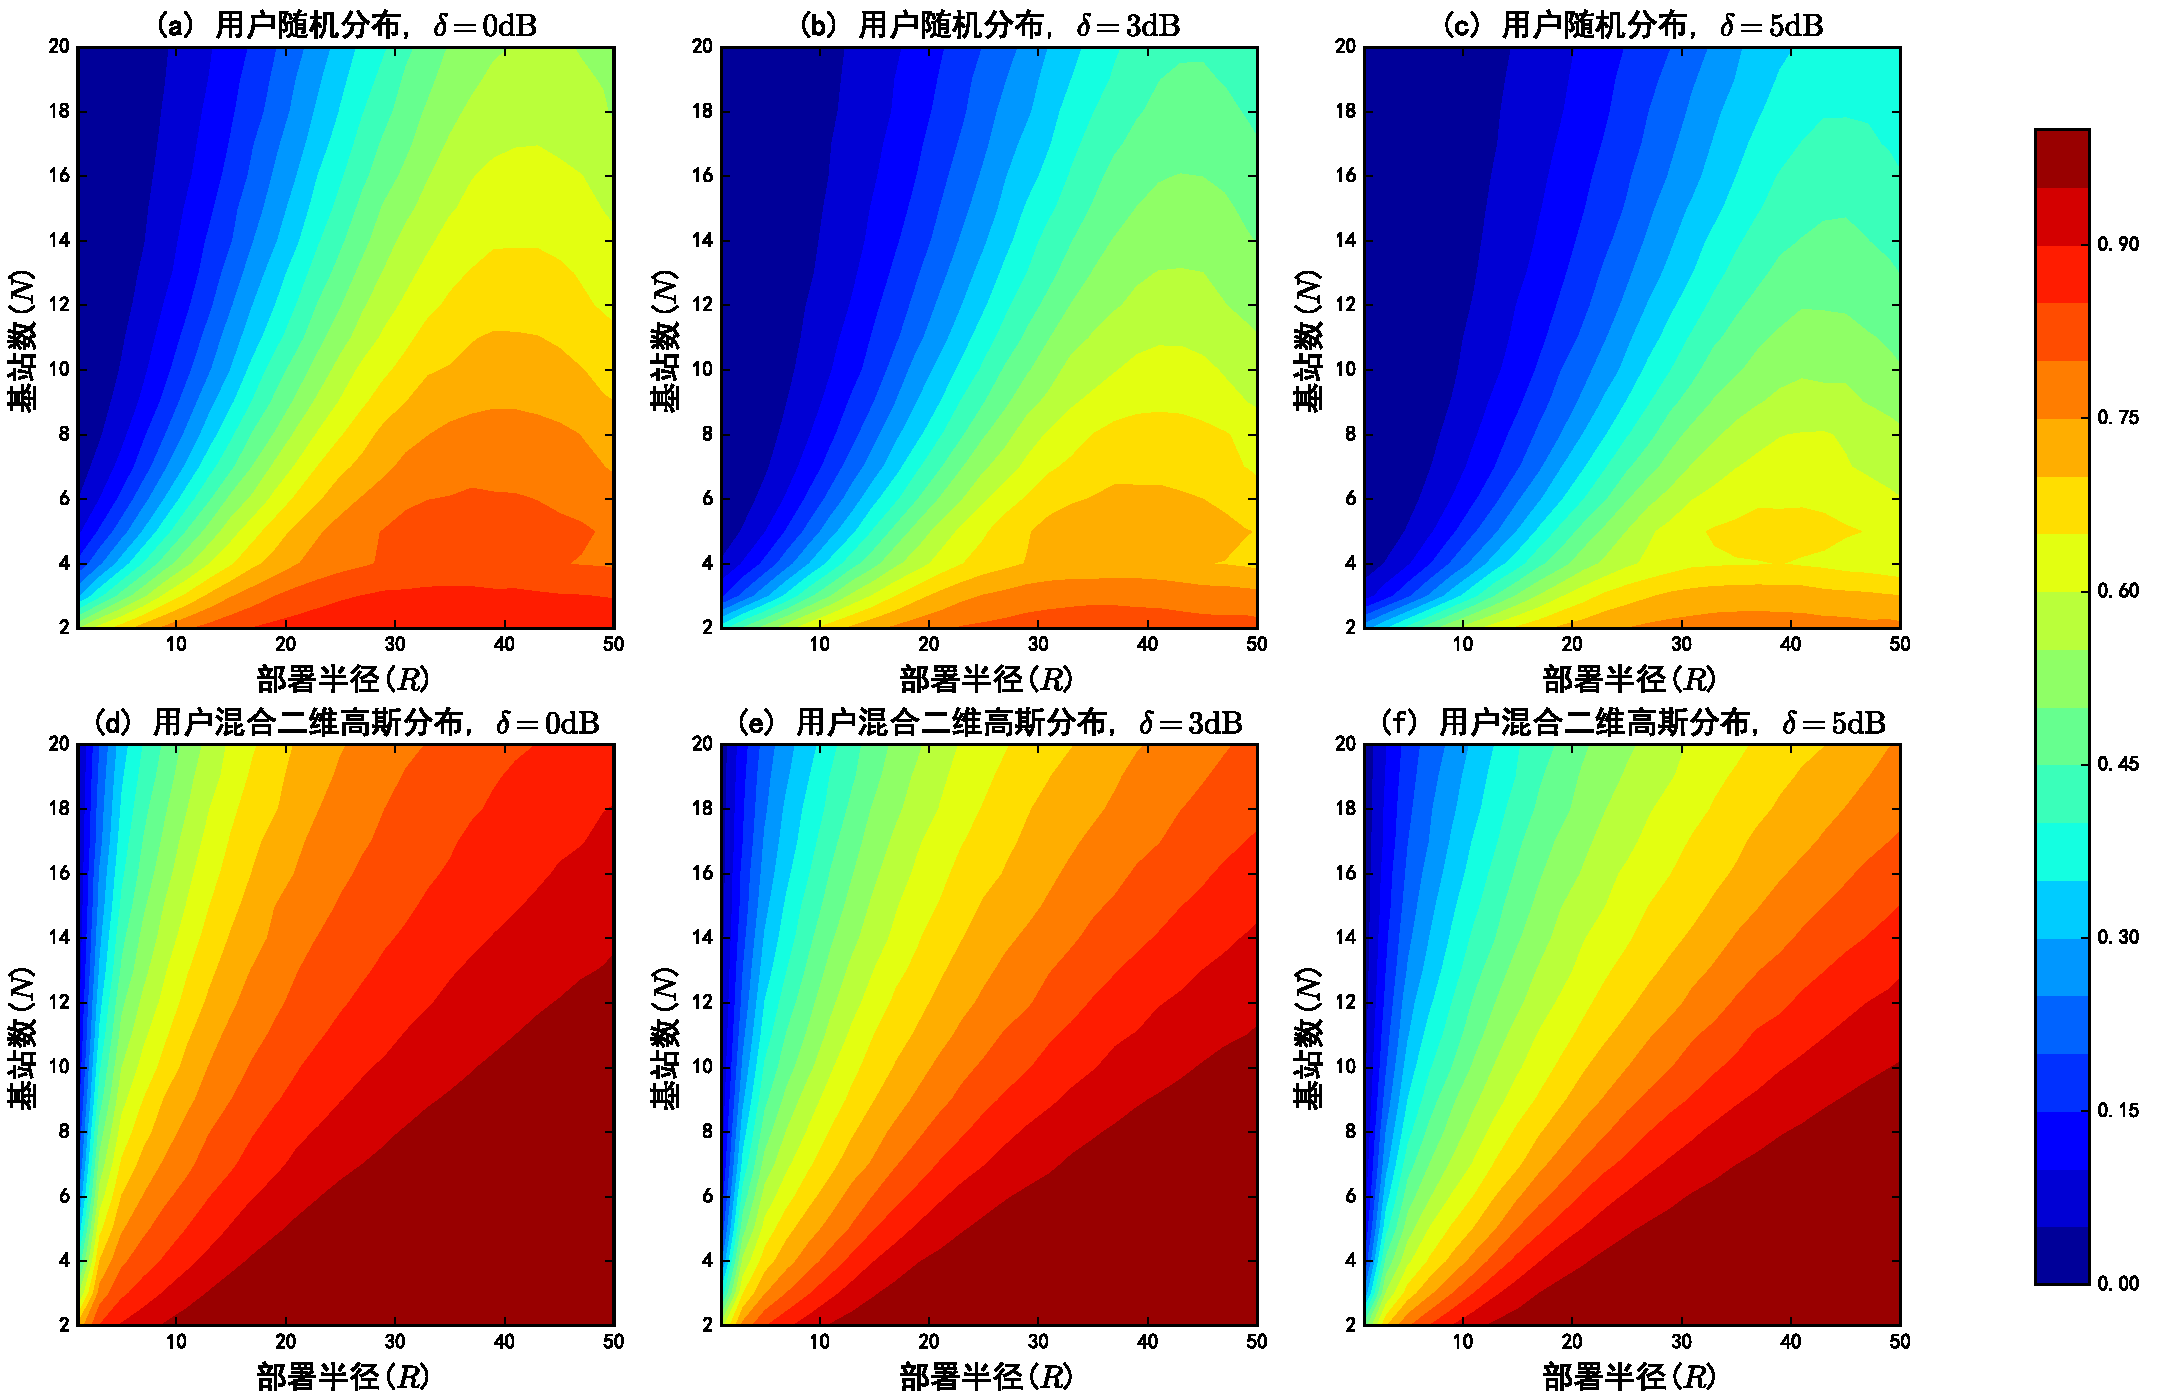
\includegraphics[width = 0.98\textwidth]{pc_random_single_circle_r_n_face.pdf}
\caption{环形基站部署的覆盖率受基站数和部署半径的影响}\vspace{-0.5em}
\label{pc_random_single_circle_r_n_face}
\end{figure}

\BiSubsection{环形基站部署的单位面积频谱效率的分析}{Defination of UDNs}

在前面的小节中,我们讨论了环形基站部署的覆盖率的性能,其是网络的可靠性的一个重要的衡量指标,
在任何的通信系统中,用户的接收信干比都需要满足一个门限值~$\delta$~才能进行可靠的通信。
然而通信的系统不能只满足有效性要求,还需要满足可靠性的要求。
衡量可靠性的一个重要的指标就是频谱效率。
但在超密集组网的环境下,由于接入用户的数量较多,用户的速率需求较大,
因此,频谱效率已经不能完全满足衡量网络的有效性的要求,
需要考虑能够同时服务多少个用户,并且让用户的和速率尽可能的大,
即要求网络的单位面积频谱效率高。

本小节对环形基站部署的网络的单位面积频谱效率进行仿真,仿真的参数如表~\ref{single_circle_ase_para}~所示,
\begin{table}[htbp]
\caption{覆盖率与~$R$~和~$N$~的关系的仿真参数}
\label{single_circle_ase_para}
\vspace{0.5em}\centering\wuhao
\begin{tabular}{cccc}
\toprule[1.5pt]
参量 & & & 设置 \\
\midrule[0.5pt]
区域~$\mathcal{D}$~的大小  & & & ~$100\mathrm{m} \times 100 \mathrm{m}$ \\
信道的类型 & & &  瑞利衰落信道\\
基站的个数~$N$~ & & &  $2\sim20$\\
圆环的半径~$R$~ & & &  $1.0\sim 50\mathrm{m}$\\
用户的分布~$\Psi$~ & & & 随机分布,二维高斯分布\\
二维高斯分布的标准差~$\sigma$~ & & & ${5\mathrm{m}}$\\
信道衰落系数~$\alpha$~  & & & 4.0\\
\bottomrule[1.5pt]
\end{tabular}
\end{table}
讨论部署半径~$R$~和基站个数~$N$~对网络的单位面积频谱效率的影响,
得到的结果如图~\ref{single_circle_ase_show}~所示,
无论是用户为随机分布还是用户为以基站为均值的混合二维高斯分布,
区域的单位面积频谱效率随着部署半径~$R$~的增加而增大,
这与网络的覆盖率的性能随着~$R$~的变化规律相同,
区域的单位面积频谱效率随着基站数~$N$~的增多,
区域的单位面积频谱效率的性能逐渐变好,
这与覆盖率性能随着~$N$~的变化相反。
可以看到~$N$~增大,网络中的用户的干扰增强,
覆盖率变差,但是随之可以服务的用户增多,单位面积频谱效率变大,
在确定基站的个数的问题上反映出了通信中可靠性和有效性的矛盾。
将用户为随机分布和混合二维高斯分布的单位面积频谱效率性能作对比,
由于在用户为混合二维高斯分布条件下,距离基站近的用户较之于用户为随机分布下更多,
因此其覆盖率性能和单位面积频谱效率的性能均更好。
\begin{figure}[htbp]
\centering
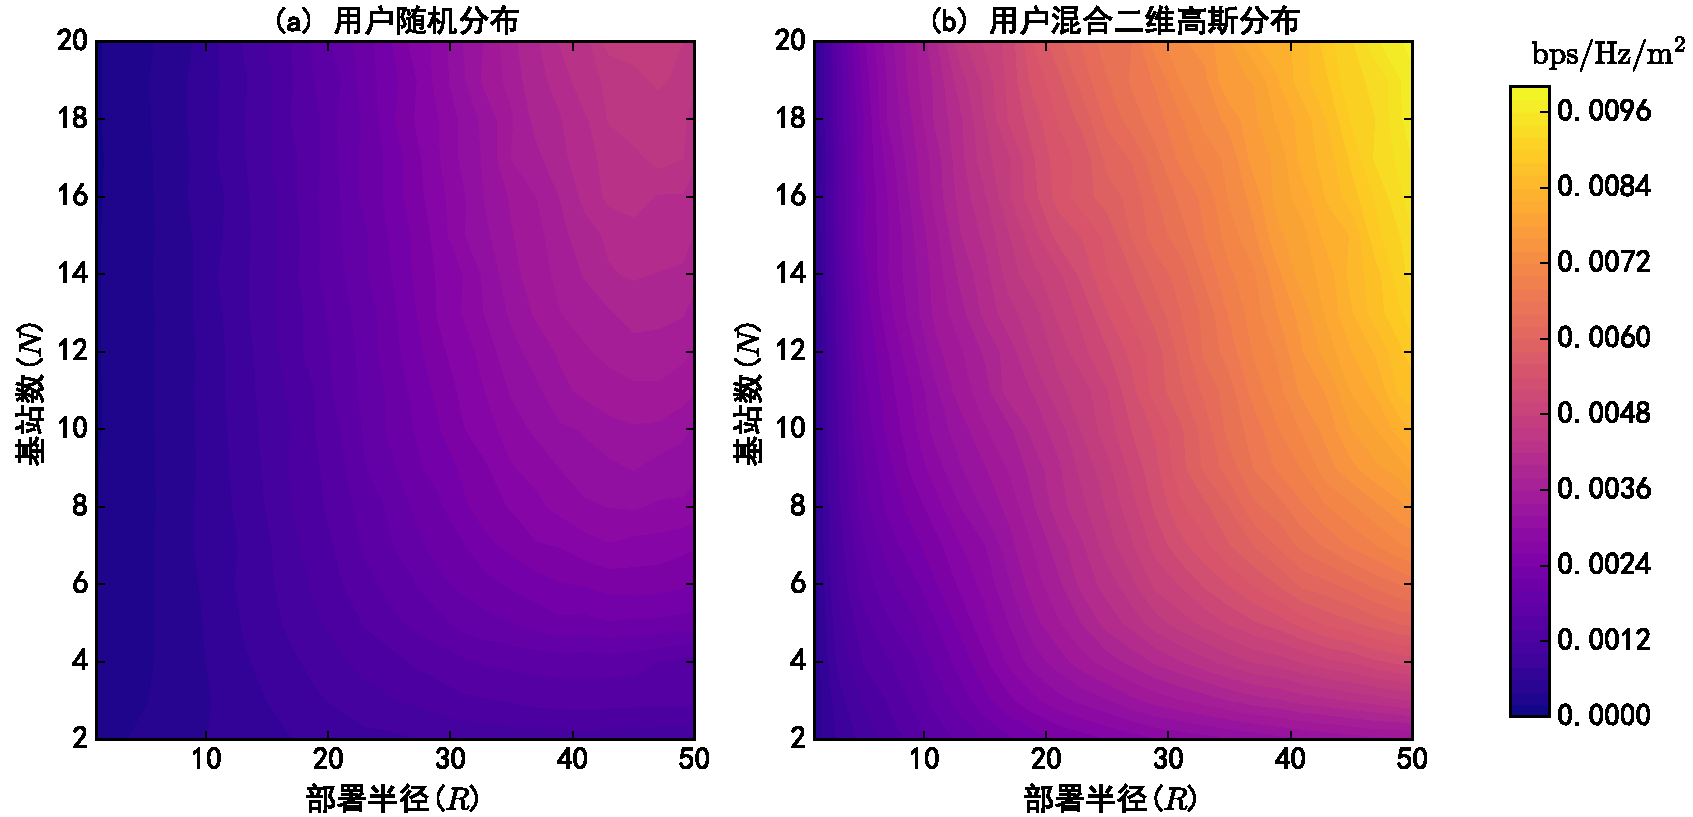
\includegraphics[width = 0.90\textwidth]{single_circle_ase_show.pdf}
\caption{环形基站部署的单位面积频谱效率受基站数和部署半径的影响}\vspace{-0.5em}
\label{single_circle_ase_show}
\end{figure}

\BiSection{方格形的基站部署的覆盖率的性能分析}{Defination of UDNs}
\BiSubsection{方格形的基站部署的拓扑结构}{Defination of UDNs}
方格形的基站部署将基站部署在固定的方格点上,部署的方法为首先在区域内的纵向每隔~$l_1$~画一条直线,
然后在横向每隔~$l_2$~画一条之间,将基站部署在直线的相交点上。
方格形的基站部署方法的示意图如图~\ref{grid_bs_station_show}~所示,
\begin{figure}[htbp]
\centering
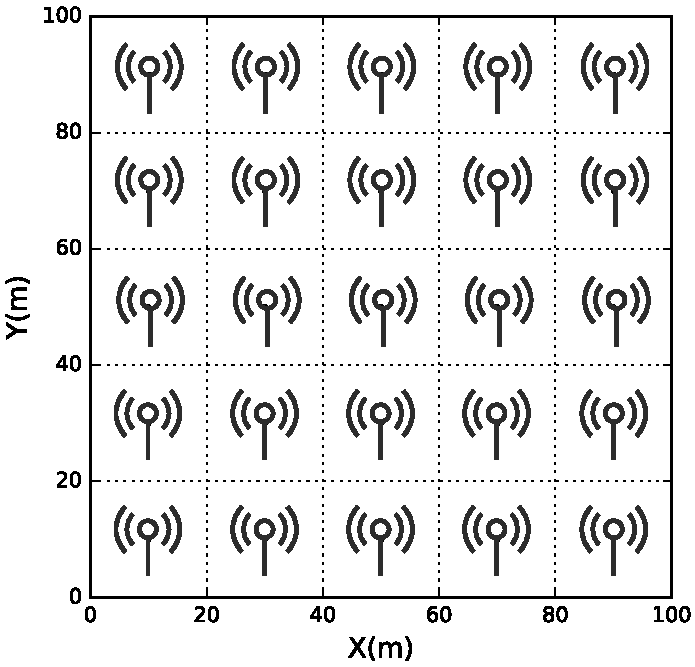
\includegraphics[width = 0.62\textwidth]{grid_bs_station_show.pdf}
\caption{方格形基站部署的拓扑结构示意图}\vspace{-0.5em}
\label{grid_bs_station_show}
\end{figure}
在图~\ref{grid_bs_station_show}~所示的基站拓扑结构中,区域~$\mathcal{D}$~为为一个~$100\mathrm{m}\times 100 \mathrm{m}$~的区域,
$l_1=l_2=20\mathrm{m}$,
在横向和纵向上均每隔~$20\mathrm{m}$~部署一个基站,一共在区域内共部署了~25~个基站。
再该场景下基站均匀的部署在了区域内,每个基站的负载均衡,每隔微基站覆盖的区域的性能相同,适合区域内用户均匀分布的情况。
但在未采用协作的情况下,用户选择距离其最近的基站作为服务基站,因此在小区边缘的用户受到的干扰较强,
边缘用户的覆盖率和遍历容量较差。
下面对在不同的参数条件下的基站格点形部署的性能进行定性和定量的分析。

\BiSubsection{方格形的基站部署的遍历容量}{Defination of UDNs}
对方格形基站的遍历容量分布图进行蒙特卡洛仿真分析,
仿真的参数表如表~\ref{square_grid_sinr_sim_para}~所示,
\begin{table}[htbp]
\caption{遍历容量的热力分布图的仿真参数}
\label{square_grid_sinr_sim_para}
\vspace{0.5em}\centering\wuhao
\begin{tabular}{cccc}
\toprule[1.5pt]
参量 & & & 设置 \\
\midrule[0.5pt]
区域~$\mathcal{D}$~的大小  & & & ~$100\mathrm{m} \times 100 \mathrm{m}$~ \\
横向间隔$l_1$~ & & &  ${20\mathrm{m}}$\\
纵向间隔$l_2$~ & & &  ${20\mathrm{m}}$\\
信道衰落系数~$\alpha$~  & & & 2,~4\\
\bottomrule[1.5pt]
\end{tabular}
\end{table}
对网络的各个位置,每个位置采用蒙特卡洛仿真,对每个位置的遍历容量进行仿真,
得到遍历容量的热力分布图如图~\ref{square_grid_e_capacity_show}~所示。
\begin{figure}[htbp]
\centering
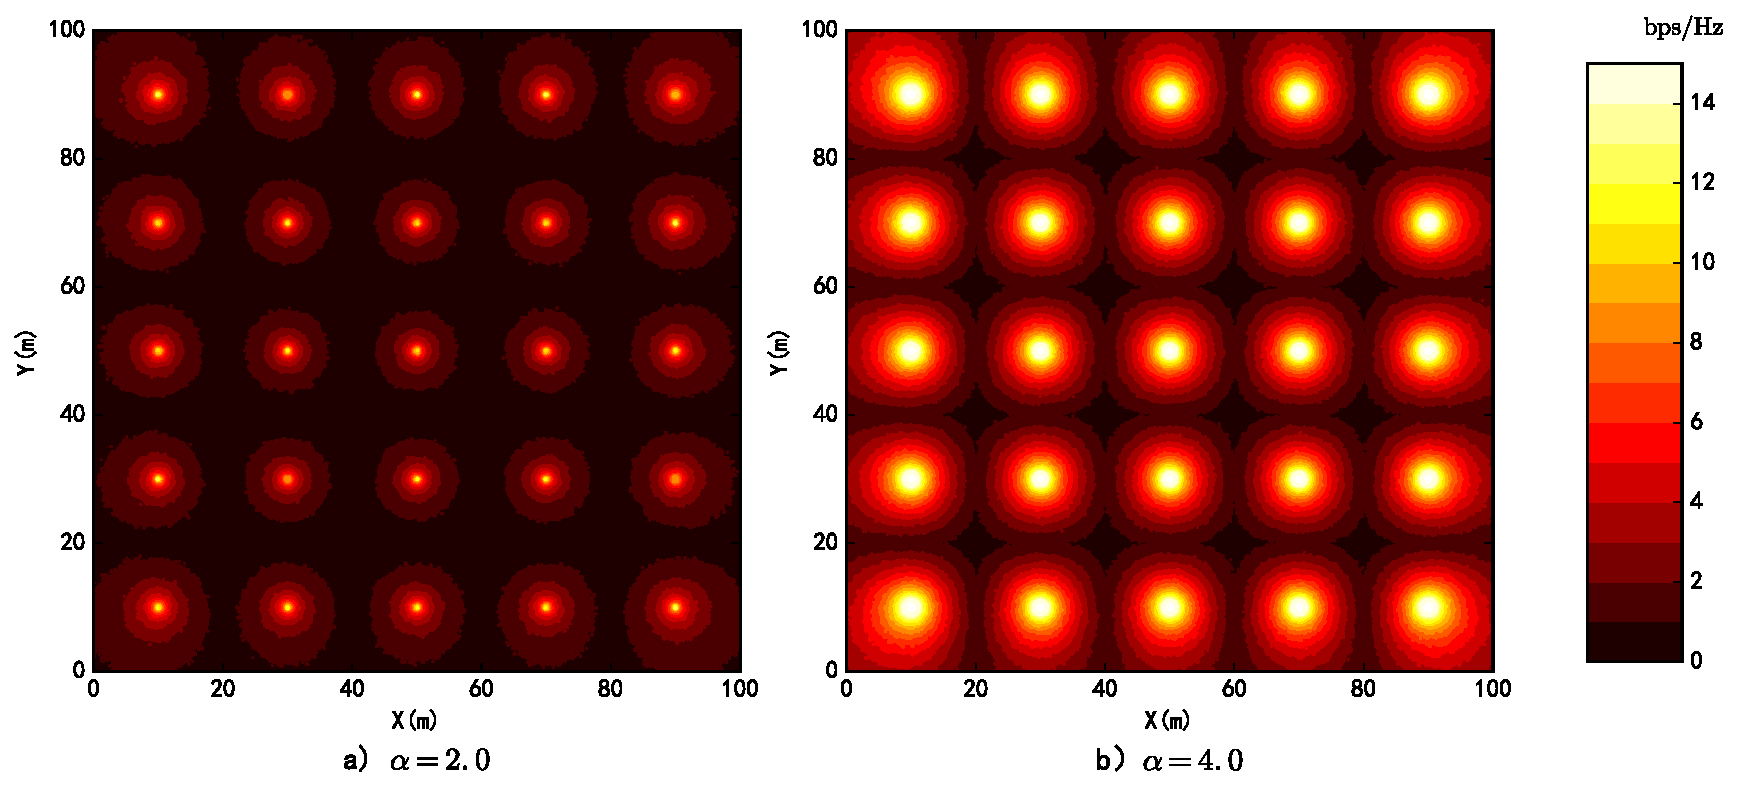
\includegraphics[width = 0.90\textwidth]{square_grid_e_capacity_show.pdf}
\caption{方格形基站部署的遍历容量热力图}\vspace{-0.5em}
\label{square_grid_e_capacity_show}
\end{figure}
可以看到较环形区域的遍历容量的热力图比较,
对于~$\alpha=2.0$~的情况,大约有超过一半的区域的遍历容量大于~$1\mathrm{bps/Hz}$,
对于~$\alpha=4.0$~的情况,大部分区域的遍历容量大于~$1\mathrm{bps/Hz}$。
与环形的基站部署的热力分布图不同,
网络中没有大面积的性能较差的区域,取而代之的是在每相互接壤的四个基站的中心处,
由于受到干扰基站的强烈的干扰,网络的遍历容量性能较差,小于~$1\mathrm{bps/Hz}$。
虽然大部分区域的覆盖率性能较好,但是仍然需要对基站中心的用户采用技术手段对其性能进行提升。

\BiSubsection{方格形的基站部署的覆盖率}{Defination of UDNs}
我们在上一小节对网络的遍历容量进行了定性的分析,
下面对网络的覆盖率性能做定量的分析,
主要分析在不同的横纵间隔~$l_1$、$l_2$~的情况下,基站的覆盖率的性能。
也对不同用户的分布情况下网络的覆盖率的性能进行了定量的分析,
考虑用户的分布~$\Psi$~分别为随机分布和混合二维高斯分布的情况。
仿真的参数表如表~\ref{square_grid_pc_sim_para}~所示,
\begin{table}[htbp]
\caption{覆盖率的仿真参数}
\label{square_grid_pc_sim_para}
\vspace{0.5em}\centering\wuhao
\begin{tabular}{cccc}
\toprule[1.5pt]
参量 & & & 设置 \\
\midrule[0.5pt]
区域~$\mathcal{D}$~的大小  & & & ~$100\mathrm{m} \times 100 \mathrm{m}$ \\
基站的横向间隔~$l_1$~ & & &  $10\mathrm{m} , 20\mathrm{m}$ \\
基站的纵向间隔~$l_2$~ & & &  $10\mathrm{m} , 20\mathrm{m}$ \\
用户的分布~$\Psi$~ & & & 随机分布,二维高斯分布\\
二维高斯分布的标准差~$\sigma$~ & & & ${5\mathrm{m}}$\\
信道衰落系数~$\alpha$~  & & & 4.0\\
\bottomrule[1.5pt]
\end{tabular}
\end{table}

对所给定的横纵间隔进行组合,
对~$l_1=10\mathrm{m},~l_2=10\mathrm{m}$,$l_1=10\mathrm{m},~l_2=20\mathrm{m}$,
$l_1=10\mathrm{m},~l_2=20\mathrm{m}$~3~种情况进行分析,覆盖率性能的曲线如图
~\ref{pc_random_square_gird_l12}~所示,在途中可以看到,当用户的分布服从随机分布的情况下,
不同的基站的横纵间隔~$l_1$~和~$l_2$~对网络的覆盖率性能影响不大,
随着基站之间的距离逐渐边远,网络的覆盖率性能逐渐变好,
由于基站之间的距离不断地边远,干扰信号的强度更低,得到的覆盖率性能也更好,
这也可以看出随着基站密度的下降,网络的覆盖率性能提升了。
在~$l_1=l_2=10\mathrm{m}$~的情况下,网络的~$5~\mathrm{dB}$~的覆盖率性能为~0.6。
而当用户的分布为混合二维高斯分布的情况下,
可以看到在~$l_1=l_2=10\mathrm{m}$~时得到的曲线的覆盖率相较于其他曲线的性能有较大的提升,
因为我们假设用户分布的标准差为~$5~\mathrm{m}$,而当间隔超过~$20~\mathrm{m}$~后,
即四个标准差,网络中的用户处于边缘的概率就很小了,因此覆盖率有了显著的提升。
\begin{figure}[htbp]
\centering
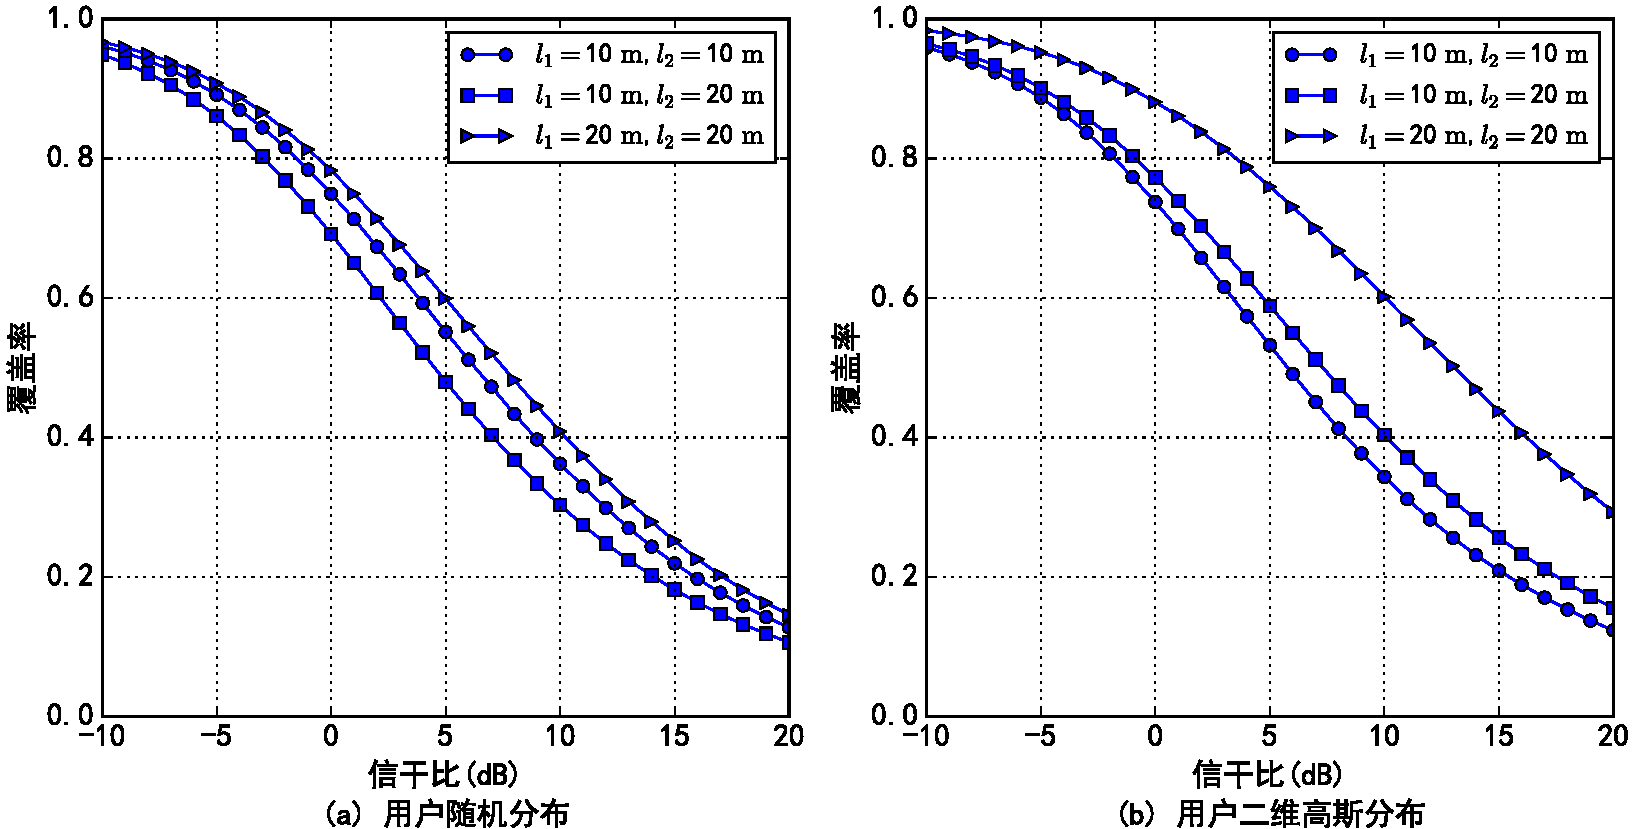
\includegraphics[width = 0.90\textwidth]{pc_random_square_gird_l12.pdf}
\caption{环形基站部署的覆盖率性能曲线}\vspace{-0.5em}
\label{pc_random_square_gird_l12}
\end{figure}
选定信干比的值为~$0\mathrm{dB}$,$3\mathrm{dB}$~和~$5\mathrm{dB}$~时,
可以得到覆盖率与~$l_1$~和~$l_2$~的关系曲面图,仿真的参数如表~\ref{square_grid_pc_para}~所示,
\begin{table}[htbp]
\caption{覆盖率与~$l_1$~和~$l_2$~的关系的仿真参数}
\label{square_grid_pc_para}
\vspace{0.5em}\centering\wuhao
\begin{tabular}{cccc}
\toprule[1.5pt]
参量 & & & 设置 \\
\midrule[0.5pt]
区域~$\mathcal{D}$~的大小  & & & ~$100\mathrm{m} \times 100 \mathrm{m}$ \\
基站的横向间隔~$l_1$~ & & &  $5.0\sim 25.0\mathrm{m}$\\
圆环的纵向间隔~$l_2$~ & & &  $5.0\sim 25.0\mathrm{m}$\\
用户的分布~$\Psi$~ & & & 随机分布,二维高斯分布\\
二维高斯分布的标准差~$\sigma$~ & & & ${5\mathrm{m}}$\\
信道衰落系数~$\alpha$~  & & & 4.0\\
\bottomrule[1.5pt]
\end{tabular}
\end{table}
得到的仿真曲面图如图~\ref{pc_l1_l2}~所示,通过仿真图的结果可以看出,
在同样的基站之间的距离的情况下,
基站的的横向间距和纵向间距越是接近,其覆盖率就更高,无论是用户为随机分布还是用户为高斯分布,
均是随着距离的增加,覆盖率的性能是逐渐提高的,和之前的仿真曲线得到的分析结果基本一致。
本小节对基于方格形的基站部署方法的覆盖率性能做了仿真分析,其中通过在给定网络
的拓扑结构的情况下,对网络的覆盖率性能的定量得分析,
\begin{figure}[htbp]
\centering
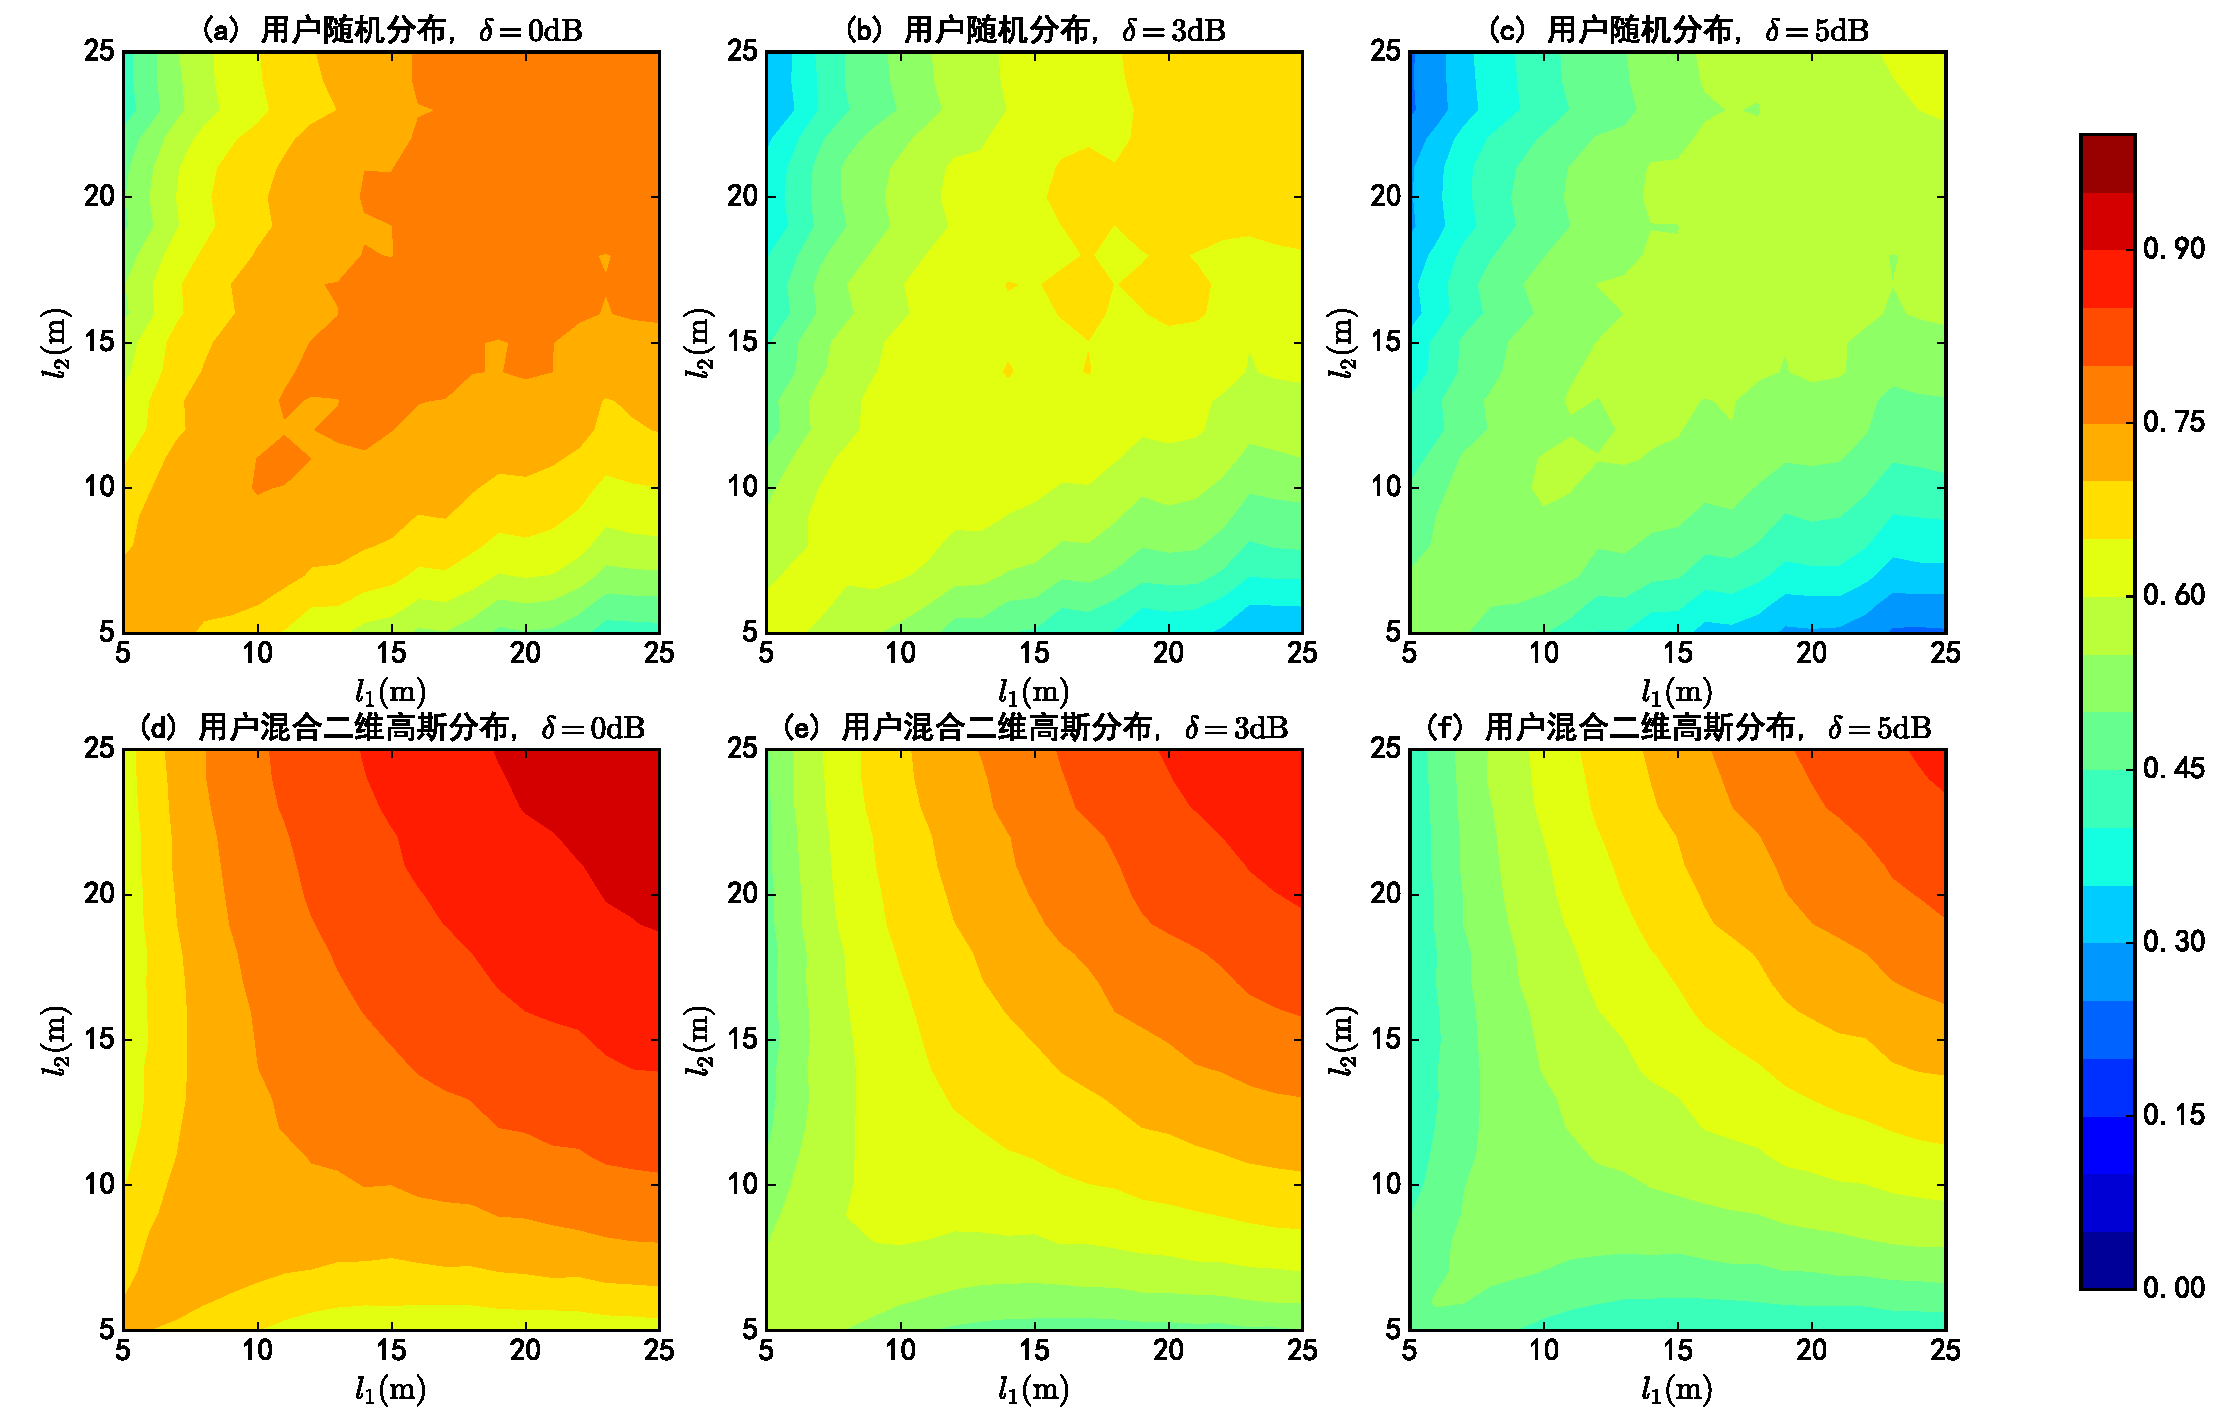
\includegraphics[width = 0.98\textwidth]{pc_l1_l2.pdf}
\caption{环形基站部署的覆盖率受基站数和部署半径的影响}\vspace{-0.5em}
\label{pc_l1_l2}
\end{figure}
可以看到覆盖率在用户为随机分布的情况下,随距离的覆盖率的提升不明显,
但当为二维高斯分布的情况下,随着距离逐渐增大,网络的覆盖率有明显的提升,
从通过颜色反映出来的图的梯度特性上可以看出,当基站之间的距离较小时,单独增加横或者纵的距离,可能会使网络的覆盖率的性能下降。
接着我们对网络中覆盖率受到基站间隔的影响进行了分析,得出当横纵间距相等时,覆盖率是距离的单调递增函数,
说明距离边远,对用户接收干扰的影响大于对用户接收有用功率的影响。


\BiSubsection{方格形的基站部署的单位面积谱效率}{Defination of UDNs}

本小节对方格形基站部署的网络的单位面积频谱效率进行仿真,仿真的参数如
表~\ref{grid_ase_param}~所示,
\begin{table}[htbp]
\caption{单位面积谱效率与~$l_1$~和~$l_2$~的关系的仿真参数}
\label{grid_ase_param}
\vspace{0.5em}\centering\wuhao
\begin{tabular}{cccc}
\toprule[1.5pt]
参量 & & & 设置 \\
\midrule[0.5pt]
区域~$\mathcal{D}$~的大小  & & & ~$100\mathrm{m} \times 100 \mathrm{m}$ \\
基站横向间距~$l_1$~ & & &  $5.0\sim 25.0\mathrm{m}$\\
基站纵向间距~$R$~ & & &  $5.0\sim 25.0\mathrm{m}$\\
用户的分布~$\Psi$~ & & & 随机分布,二维高斯分布\\
二维高斯分布的标准差~$\sigma$~ & & & ${5\mathrm{m}}$\\
信道衰落系数~$\alpha$~  & & & 4.0\\
\bottomrule[1.5pt]
\end{tabular}
\end{table}
讨论基站的横向距离~$l_1$~ 和基站的纵向距离~$l_2$~对网络的单位面积频谱效率的影响,得
到的结果如图~\ref{grid_ase_show}~所示,
可以看到基站的距离越近,区域内基站的密度越高,其单位面积频谱效率就越好,
得到了和覆盖率性能完全相反的结果,说明在方格形基站部署的情况下,
反应可靠性的覆盖率和反应有效性的单位面积谱效率同样是一对折中。
\begin{figure}[htbp]
\centering
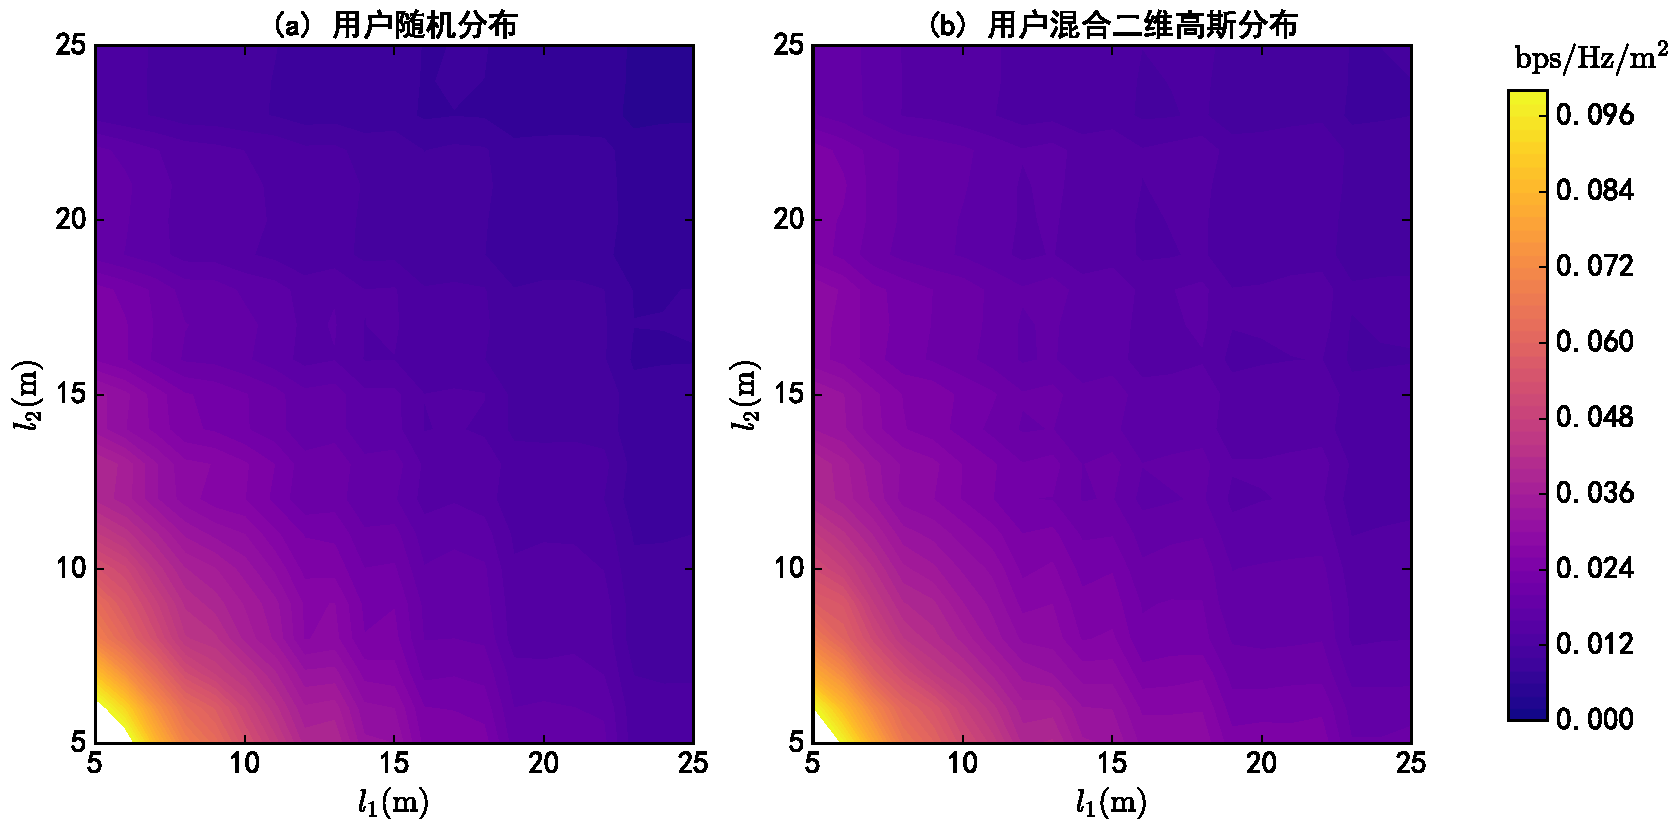
\includegraphics[width = 0.90\textwidth]{grid_ase_show.pdf}
\caption{方格形基站部署单位面积谱效率受格形的影响}\vspace{-0.5em}
\label{grid_ase_show}
\end{figure}

\BiSection{本章小结}{Conclusion}
本章主要介绍了网络的性能指标和基于格的基站部署的性能,
其中性能指标主要包括遍历容量,覆盖率和单位面积谱效率,
同时也对基于格的基站部署的性能进行了分析,包括环形基站的拓扑结构和方格形基站的拓扑结构。
